%!TEX root = ../template.tex
%%%%%%%%%%%%%%%%%%%%%%%%%%%%%%%%%%%%%%%%%%%%%%%%%%%%%%%%%%%%%%%%%%%%
%% chapter4.tex
%% NOVA thesis document file
%%
%% Chapter with lots of dummy text
%%%%%%%%%%%%%%%%%%%%%%%%%%%%%%%%%%%%%%%%%%%%%%%%%%%%%%%%%%%%%%%%%%%%

\typeout{NT FILE chapter4.tex}%

\chapter{Problem Definition and Scope}
\label{cha:definition}

This thesis tackles two key challenges in the assembly of HPC (High Pressure Compressor) blades. The goal is to ensure that the assembly process meets the required specifications and to better understand how blade geometry impacts engine performance.

The first challenge is to develop a process or tool that guarantees the correct assembly clearance for the blades. This clearance must comply with the specifications outlined in the engine manual, ensuring that the blades are assembled properly and function as intended.

The second objective is to create a reliable method for measuring the chord length of the blades and analyzing its correlation with engine performance in bench tests. By understanding this relationship, we can gain valuable insights into how small variations in manufacturing affect overall efficiency and explore ways to optimize the assembly process. Ultimately, this aims to guarantee and control engine performance according to operational needs.

Together, these objectives shape the scope of this work, which involves designing measurement tools, validating methodologies, and bridging the gap between manufacturing precision and engine performance.

In this chapter, the details of these challenges will be explored, along with the initial requirements and decisions that guided the approach taken. This will provide a comprehensive understanding of the context, constraints, and considerations that influenced the development of solutions throughout the project.

\section{Blade Assembly Process and Clearance Requirements}
\label{sec: bladeandclearence}

This study focuses on the assembly of HPC stages 6 to 10, represented in Figure~\ref{fig:hpcass},  as these are the stages that incorporate the blades under analysis, as previously mentioned. The assembly of \gls{HPC} blades follows a standardized procedure to ensure precise positioning and compliance with the required specifications. The process begins with preparing the spool, where blade slots and wire seal grooves are cleaned and inspected. Contaminants are removed to ensure a smooth surface for blade insertion. Wire seals are then installed in the grooves, adhering to specified clearance tolerances to maintain structural integrity.

\begin{figure}[H]
    \centering
    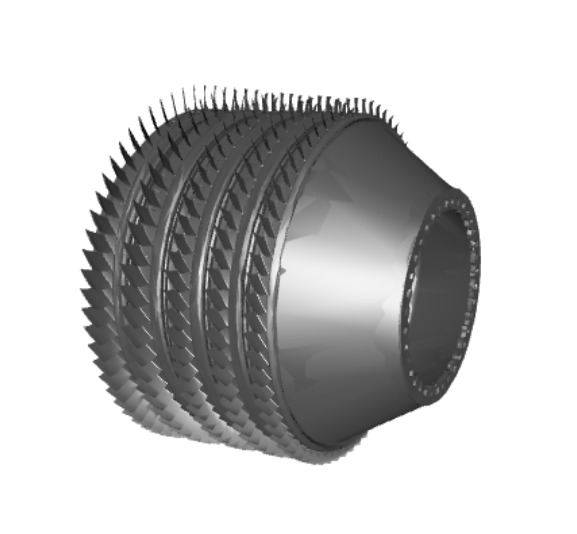
\includegraphics[width=0.5\textwidth]{hpcass.jpeg}
    \caption{\gls{LEAP}-1A \gls{HPC}.}
    \label{fig:hpcass}
\end{figure}


The blades are then inserted into the spool, following a controlled sequence to ensure a uniform distribution. During this step, each blade is checked for free movement within the dovetail slot, as any restrictions may indicate the need for replacement. After all blades are in place, locking blades are installed in designated positions to secure the assembly.

To finalize the assembly, locking lugs are positioned and their set screws are torqued to the required values. A detailed verification is performed to ensure that the locking lugs are correctly engaged within the spool’s dovetail lock slot, preventing unintended movement. To confirm the correct platform clearance, the blades are shifted in one direction to determine the maximum gap, and measurements are taken to verify compliance with the permissible range. This clearance, referred to as Clearance R, is represented in Figure~\ref{fig:assembly6}.If necessary, adjustments are made by replacing narrow-platform blades with wide-platform ones.

\begin{figure}[H]
    \centering
    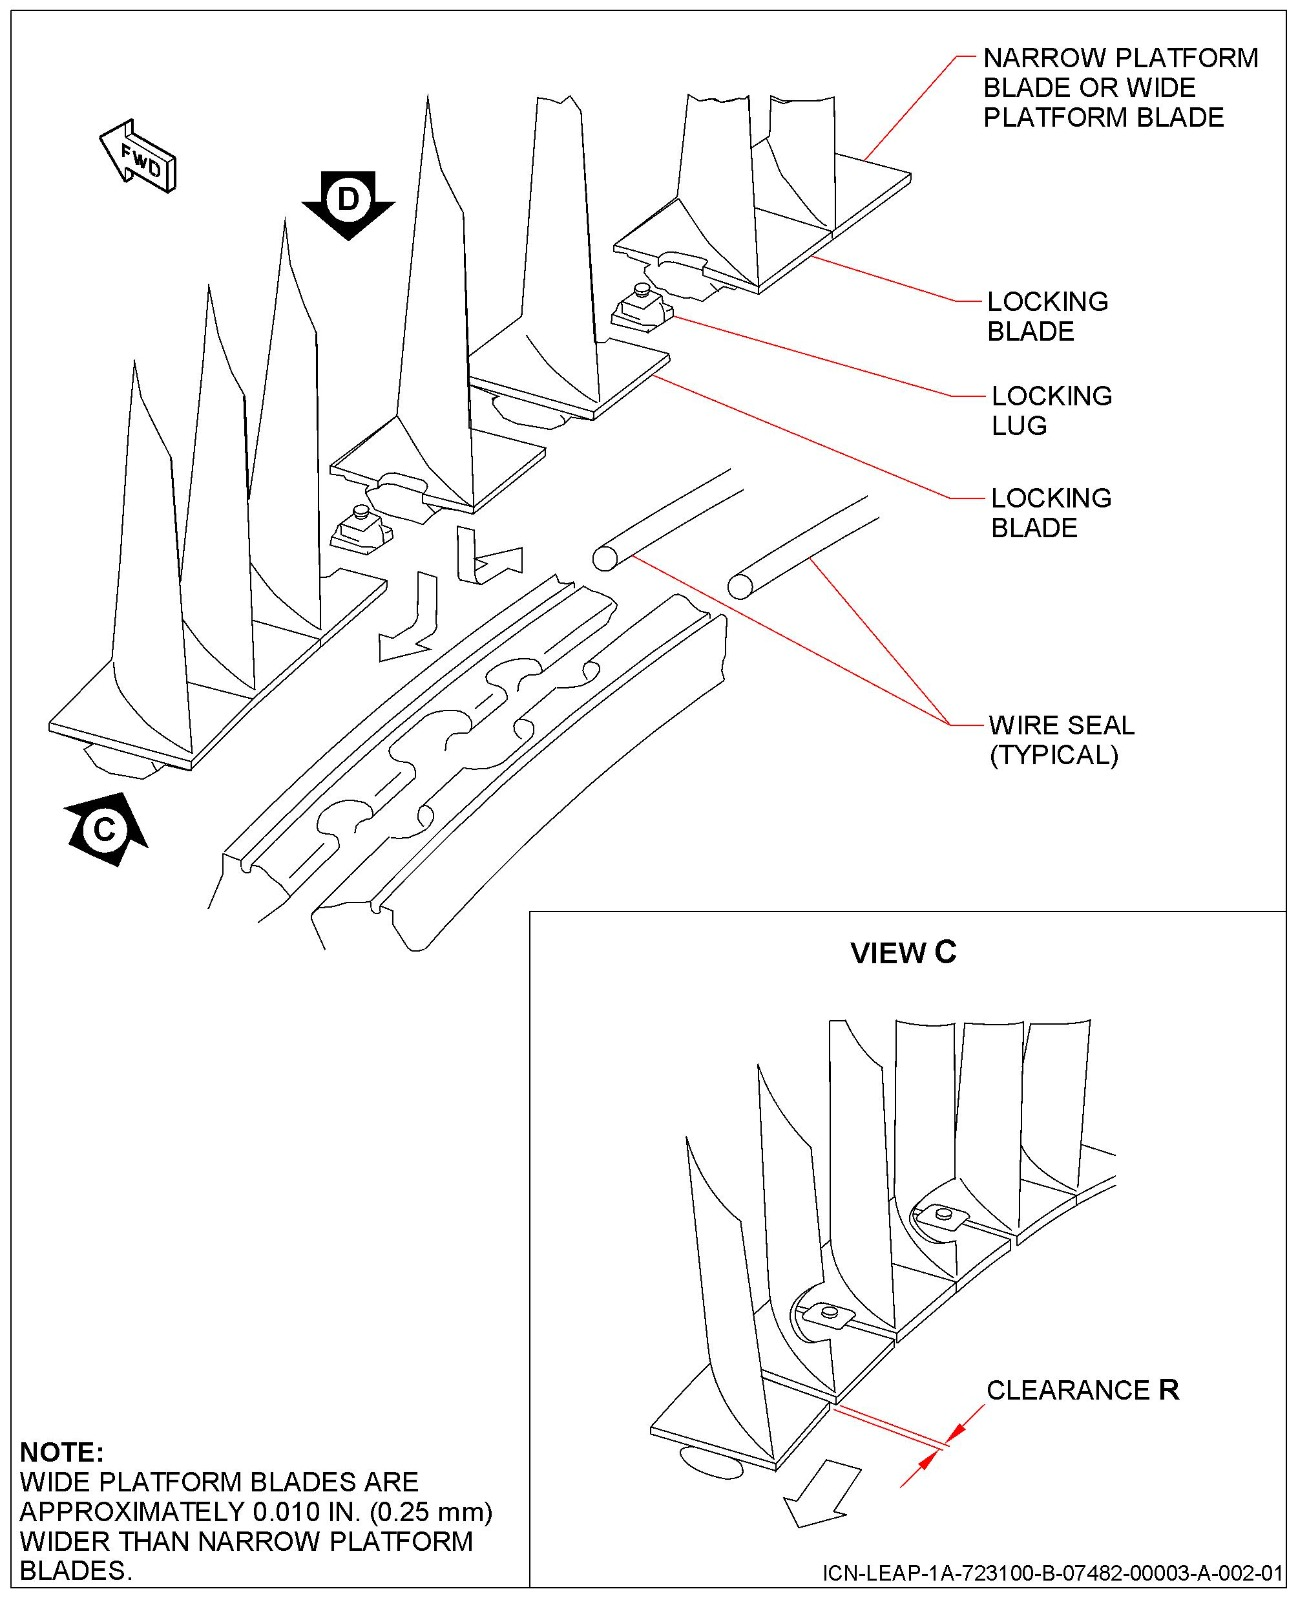
\includegraphics[width=0.5\textwidth]{assembly6.jpeg}
    \caption{Stage Components and Clearence Representation}
    \label{fig:assembly6}
\end{figure}


The measurement of the clearance is performed using a feeler gauge (with a corresponding image), ensuring precise determination of the gap. For each compressor stage, a predefined clearance value is specified, as presented in Table~\ref{tab:clearance_tolerance}. In the aviation industry, these clearance values are typically provided in inches. However, throughout the development of this dissertation, all measurements have been converted to millimeters to maintain consistency.

Once the correct blade sequence and clearance are established, the assembly is reinstalled, and a final torque check is performed on the locking lugs. Ensuring that all components remain within the prescribed limits is critical to maintaining engine performance and durability, as deviations from the specified tolerances can lead to excessive wear, unwanted vibrations, or mechanical failures.

\begin{table}[h]
    \centering
    \begin{tabular}{ccccc}
        \toprule
        Stage & \makecell{Assembly Clearance \\ Tolerance [in]} & \makecell{Assembly Clearance \\ Tolerance [mm]} & Clearance [mm]\\
        \midrule
        6  & 0.010-0.030 & 0.254-0.762  &  \\
        7  & 0.010-0.030 & 0.254-0.762  &  \\
        8  & 0.010-0.030 & 0.254-0.762  & 0.508 \\
        9  & 0.080-0.100 & 2.032-2.54   &   \\
        10 & 0.149-0.169 & 3.7846-4.2926 &  \\
        \midrule
    \end{tabular}
    \caption{Assembly clearance tolerances for different stages.}
    \label{tab:clearance_tolerance}
\end{table}

Currently, in \gls{TAP}'s \gls{ME} Engine Shop assembly process, there is no method to anticipate this clearance before the assembly stage. As a result, if the measured clearance after assembly does not fall within the required specifications, additional wide-platform blades may need to be sourced from the supplier. This can introduce delays in the workflow, as the availability of the necessary blades depends on supplier lead times. As represented in Figure~\ref{fig:assembly6}, wide-platform blades are approximately 0.25 mm wider than narrow blades, allowing for clearance adjustments when needed. Implementing a way to predict and control clearance earlier in the process would help streamline operations, reducing waiting times and improving overall efficiency.

As a first step, it is necessary to construct a nominal model of the blades from which further work can be carried out. This model will serve as the foundation for predicting and controlling assembly clearances, ensuring compliance with specifications, and improving process efficiency.

\subsection{Defining Platform Tolerances and Tolerance Analysis Model for the Blade}
\label{subsec:desafios}

One of the primary challenges in ensuring proper assembly clearance is the precision required to construct a nominal model of the blades. The assembly clearance depends on the individual blade dimensions, particularly the platform width, as these factor determine how the blades fit within the spool slots. To develop an effective process, it is essential to establish a nominal blade model with a precision level derived from the permissible clearance tolerances.

The required precision level can be derived from the assembly clearance by considering the maximum allowable variation that still maintains compliance. This ensures that the model reflects real-world manufacturing conditions and enables accurate clearance prediction.

To define the tolerance for the nominal model, a statistical approach is utilized, as described in \cite{TSM}. Unlike the total interchangeability model, where tolerances are summed linearly, the statistical model considers the probability distribution of component variations. The assembly tolerance is calculated using the following equation:

\begin{equation}
    T_{\text{conj}} = \sqrt{\sum_{i=1}^{n} t_i^2}
    \label{eq:estat}
\end{equation}

where:
\begin{itemize}
\item $T_{\text{conj}}$ - Assembly Tolerance
\item $t_i$ - Part Tolerance
\end{itemize}

This approach reduces the overall tolerance accumulation, making it more suitable for large-scale production where component variations follow a normal distribution. By applying this model, it is possible to maintain a precise nominal blade model while accommodating natural manufacturing variations.

\subsubsection{Calculation of Platform Dimensional Tolerance for Each Blade Type and Stage Using the statistical model}
\label{subsubsec:clearance_calculation1}
To evaluate the dimensional tolerance for each compressor stage, the number of wide and narrow blades assembled in the engine was analyzed. Table~\ref{tab:blade_distribution} presents the distribution of wide and narrow blades for each stage, along with the total number of blades.
The assembly data was collected from a motor assembled in the workshop to determine the exact number of blades used.
\begin{table}[h]
    \centering
    \begin{tabular}{@{}cccc@{}}
        \toprule
        Stage & Wide Blades & Narrow Blades & Total Blades \\ 
        \midrule
        6  & 26 & 36 & 62 \\ 
        7  & 24 & 33 & 57 \\ 
        8  & 24 & 39 & 63 \\ 
        9  & 23 & 37 & 60 \\ 
        10 & 26 & 39 & 65 \\ 
        \bottomrule
    \end{tabular}
    \caption{Number of wide and narrow blades per stage.}
    \label{tab:blade_distribution}
\end{table}

Using the equation \ref{eq:estat}, and considering an assembly tolerance of 0.508 mm, we analyze the case for stage 6, which has 26 wide blades and 36 narrow blades. Beign almost identical parts, its assumed that the wide body and narrow body blades present the same tolerance, \( T_w = T_n \), the equation simplifies to:

\begin{equation}
    T_{\text{conj}} = \sqrt{26T_w^2 + 36T_n^2}
\end{equation}

\begin{equation}
    T_{\text{conj}} = \sqrt{62T_w^2} = \sqrt{62} T_w
\end{equation}

Since the total assembly tolerance is given as 0.508 mm:

\begin{equation}
    0.508 = \sqrt{62} T_w
\end{equation}

Solving for \( T_w \):

\begin{equation}
    T_w = \frac{0.508}{\sqrt{62}} = 0.0646 \text{ mm}
\end{equation}

Thus, the tolerance for each blade in stage 6 is approximately **0.0646 mm**.

Based on this analysis, the clearance values were calculated. Table~\ref{tab:clearance} presents the obtained results.

\begin{table}[h]
    \centering
    \begin{tabular}{@{}ccc@{}}
        \toprule
        Stage & Clearance (mm) & Tw = Tn \\ 
        \midrule
        6  & & 0,064516065    \\ 
        7  &   & 0,067286244    \\ 
        8  & 0.508  & 0.00000 \\ 
        9  &   & 0,065582518    \\ 
        10 &   & 0,063009645    \\ 
        \bottomrule
    \end{tabular}
    \caption{Computed clearance values per stage.}
    \label{tab:clearance}
\end{table}

These calculations, derived from workshop data and statistical analysis, ensure that the clearance assessment aligns with real assembly conditions. Furthermore, they provide insight into the required precision needed to develop a nominal model that enables a feasible and applicable solution.

\subsubsection{Calculation of Platform Dimensional Tolerance for Each Blade Type and Stage Using the Total Interchangeability Model}
\label{subsubsec:clearance_calculation2}

To assess the dimensional tolerance for each compressor stage under the total interchangeability model, we assume that all blades—wide and narrow—must individually conform to the overall assembly tolerance. This approach does not take into account statistical variations and instead assumes that each blade directly contributes to the total variation without reduction factors. The total interchangeability model represents a worst-case scenario and serves as a reference to highlight its impracticality compared to statistical models.

Using the same distribution of wide and narrow blades from Table~\ref{tab:blade_distribution}, we analyze the tolerance requirement for each stage. The total tolerance allocation assumes that each blade's tolerance adds directly to the overall variation, leading to a simplified summation approach:

\begin{equation}
T_{\text{conj}} = (26 + 36) T_w = 62 T_w
\end{equation}

Given that the total assembly tolerance remains at 0.508 mm:

\begin{equation}
0.508 = 62 T_w
\end{equation}

Solving for :

\begin{equation}
T_w = \frac{0.508}{62} = 0.00819 \text{ mm}
\end{equation}

Thus, under the total interchangeability model, each blade in stage 6 would require an individual tolerance of approximately 0.00819 mm, which is significantly tighter than the 0.0646 mm derived from the statistical model.

Applying the same method to other stages yields the results presented in Table~\ref{tab:clearance_interchangeability}.

\begin{table}[h]
    \centering
    \begin{tabular}{@{}ccc@{}}
        \toprule
        Stage & Clearance (mm) &  \newline (Total Interchangeability) \\
        \midrule
        6  & 0.508 & 0.00819    \\
        7  & 0.508 & 0.00891    \\
        8  & 0.508 & 0.00806    \\
        9  & 0.508 & 0.00847    \\
        10 & 0.508 & 0.00782    \\
        \bottomrule
    \end{tabular}
    \caption{Computed clearance values per stage using total interchangeability.}
    \label{tab:clearance_interchangeability}
\end{table}

These results clearly indicate that the total interchangeability model imposes unrealistically strict tolerances on each blade, making it practically infeasible for manufacturing and assembly. This reinforces the necessity of using statistical models to optimize tolerance allocation while maintaining feasible manufacturing constraints.

As such, in this work, the statistical model was chosen as the reference for tolerance calculations, as it provides a more realistic and achievable approach while ensuring the necessary precision for assembly.

\subsection{Analysis of Measurement Equipment Accuracy for Geometric Validation}
\label{subsec:equipment_validation}

Following this analysis, the next steps involve evaluating the available equipment previously mentioned in \ref{cha:lorem_ipsum}, specifically the Creaform HandySCAN 3D scanner and the Mitutoyo Euro-C 121210 \gls{CMM}. While the application of reverse engineering using the scanner enables the creation of a model, its lower accuracy on edges may compromise the precision required to resolve the problem. Therefore, it is necessary to use the CMM to obtain the geometry with the required accuracy. Additionally, the scanner enables the development of the CMM fixture, which will be designed using knowledge from previous dissertations.

The accuracy of the available equipment is as follows:  

\begin{itemize}
    \item HandyScan accuracy: 0.001 in (0.0254 mm)
    \item Peripheral tape accuracy: 0.0005 in (0.0127 mm)
    \item CMM accuracy: 0.00001 in (0.00000254 mm)
\end{itemize}

These values highlight the significant difference in measurement precision, reinforcing the need for a combined approach to achieve the required accuracy.

It is essential to follow the golden rule of metrology, known as George Berndt's law, which states that "the measurement uncertainty should not exceed 1/10 of the tolerance of the dimension being controlled." This principle ensures that the selected measurement tools provide results with a level of precision suitable for the given tolerances.

It is important to note that the CMM at TAP is currently inoperative (INOP), and during this project, TAP proceeded with the purchase of a new machine. However, to expedite the work, a machine was made available by the R\&D department of Hanon Systems, which will allow progress in the project and facilitate the measurement of the platform profile of the blades to properly define the dimensions required for the work

Therefore, while the HandyScan may be useful for generating general models, the CMM will be the preferred equipment to ensure that the calculated tolerances, particularly values as small as 0.0646 mm (for stage 6), are met with precision. The combination of these tools will provide a robust and accurate approach to validating and controlling assembly tolerances, ensuring that the blades fit correctly and optimizing engine performance.

\subsection{Spool Measurements and Specifications}
\label{subsec:spool_measurements}

To ensure precise assembly and proper clearance for the HPC blades, it is essential to define the key dimensions of the spool. The spool serves as the foundational structure for blade installation, and its dimensions directly impact the assembly process. 

These dimensions play a crucial role in determining the fit and function of the HPC blades. The slot width and depth directly influence how securely the blades are held in place, while the groove width and depth are vital for the proper installation of wire seals.
Additionally, platform clearance values dictate the permissible gap between adjacent blades, ensuring compliance with operational specifications.

The diameter measurements were obtained using a Peripheral tape on a previously used spool. 
During the measuring process it was possible to differenciate two diferent spool diameteres per stage,$\varnothing Up$ and $\varnothing Down$, represented in Figure~\ref{fig:diam.png}.
Table~\ref{tab:diameters} presents diameters measured.

\begin{figure}[H]
    \centering
    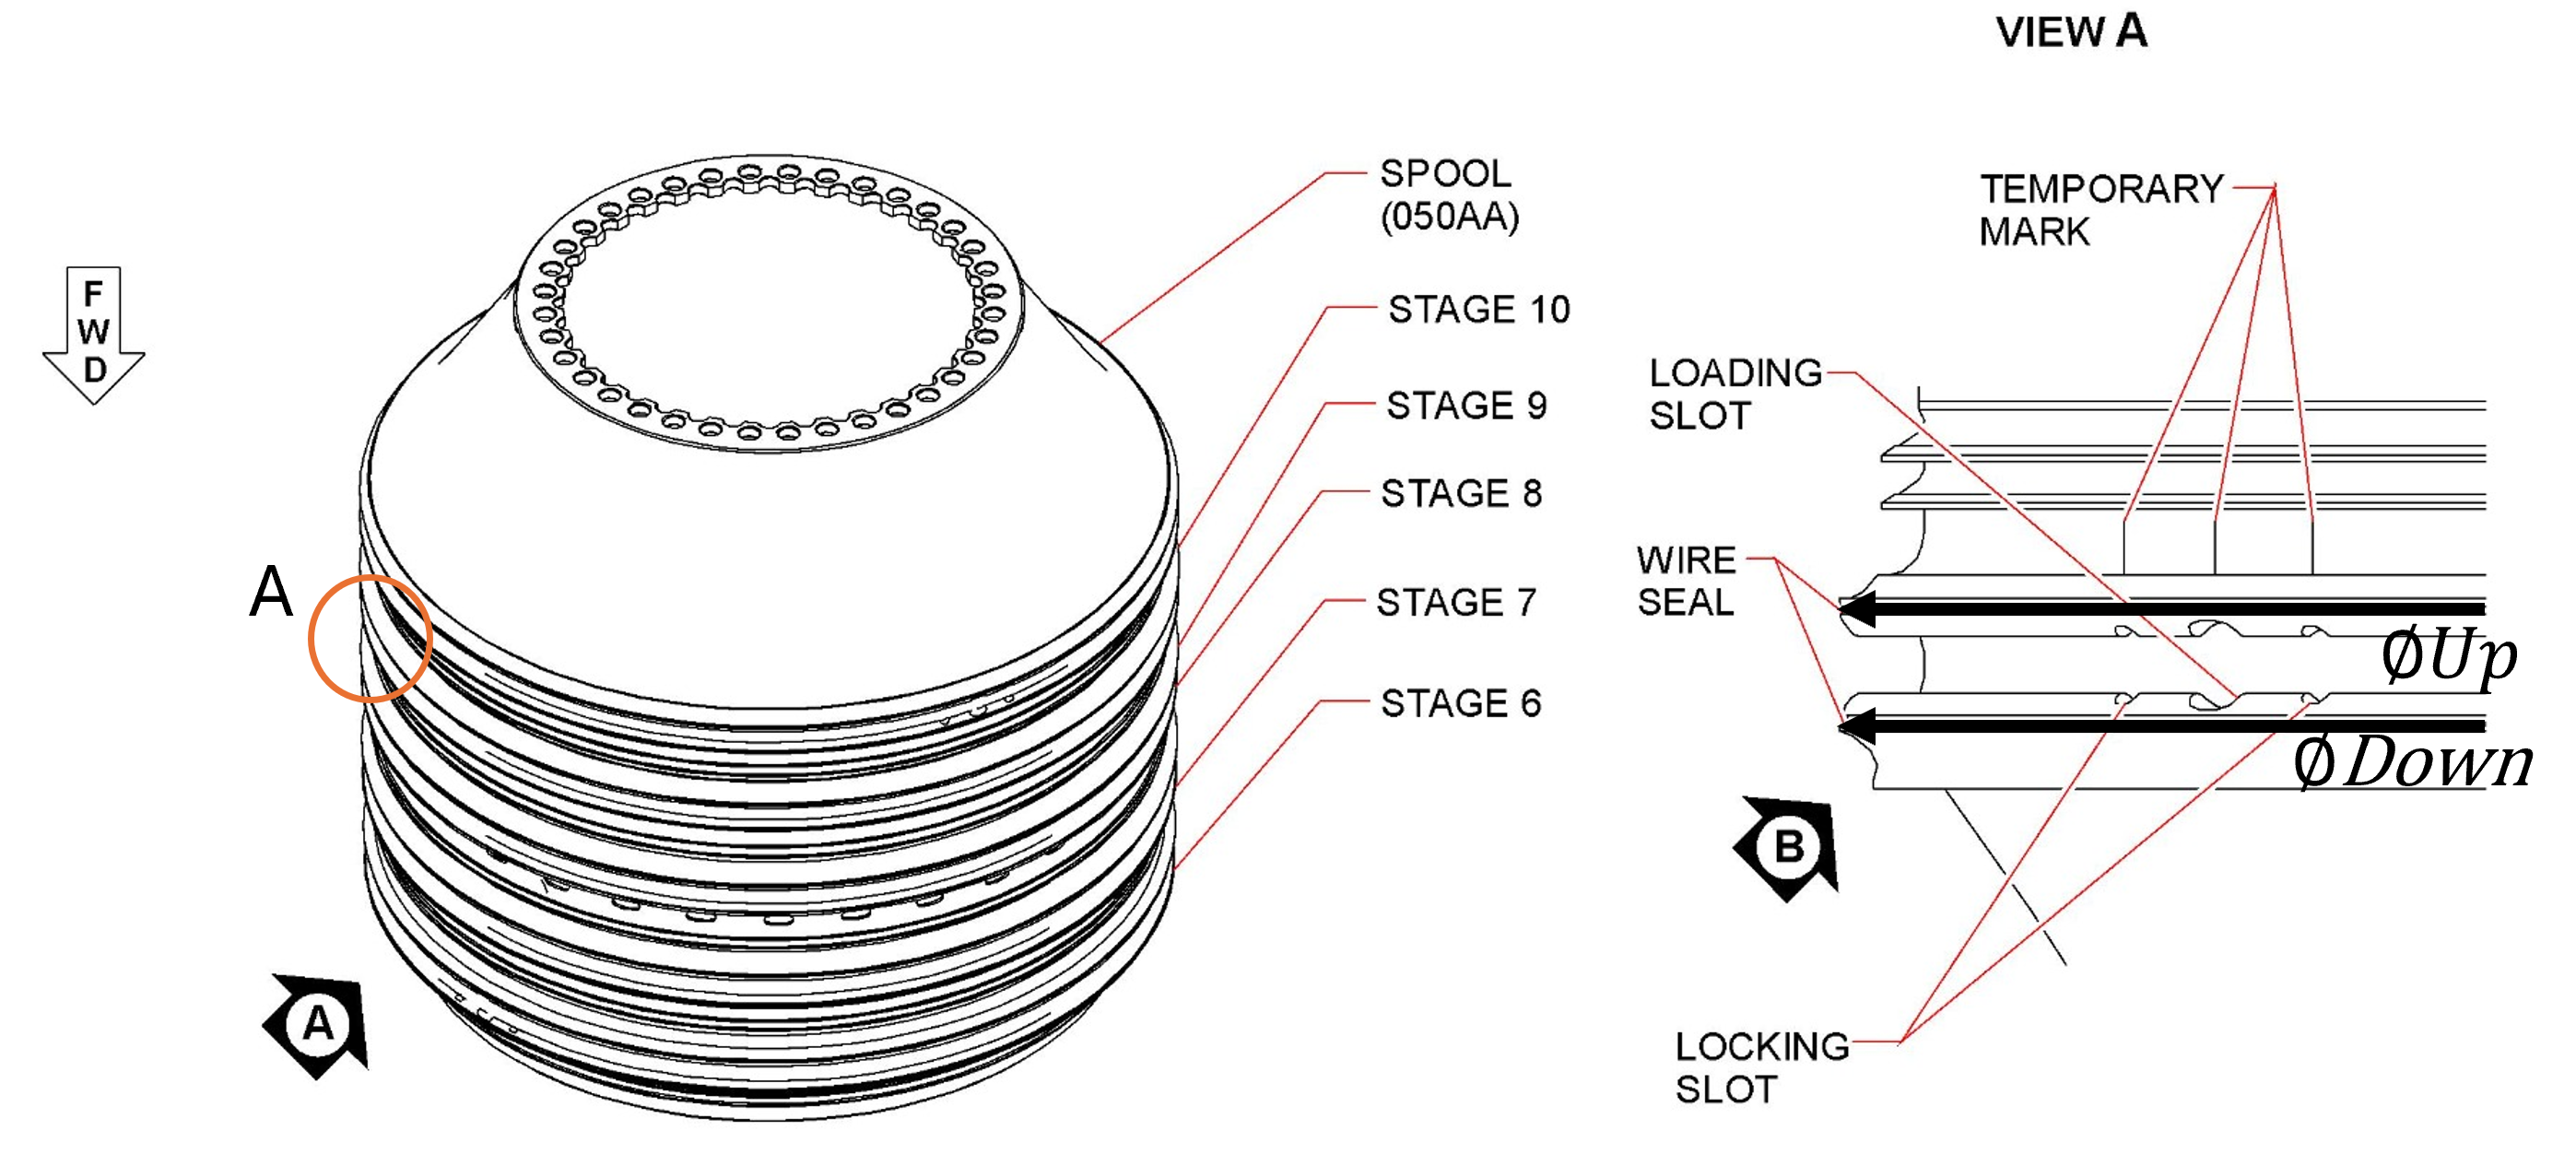
\includegraphics[width=0.8\textwidth]{diam.png}
    \caption{Stage Components and Clearence Representation}
    \label{fig:diam.png}
\end{figure}


\begin{table}[h]
    \centering
    \begin{tabular}{|c|c|c|c|c|}
        \hline
        Stage & ØUp [in] & ØDown [in] & ØUp [mm] & ØDown [mm]\\
        \hline
        10 & 15.675 & 15.69 & 398.145 & 398.526 \\
        9  & 15.704 & 15.66 & 398.882 & 397.764 \\
        8  & 15.670 & 15.62 & 398.018 & 396.748 \\
        7  & 15.620 & 15.69 & 396.748 & 398.526 \\
        6  & 15.545 & 15.52 & 394.843 & 394.208 \\
        \hline
    \end{tabular}
    \caption{Diameter values for each stage}
    \label{tab:diameters}
\end{table}

By integrating these spool measurements into the assembly process analysis, it is possible to predict and optimize the blade fitting conditions before final assembly, reducing rework and improving overall efficiency.

\subsection{Contact Point Analysis Between Blades}
\label{cha:contacto}
This section aims to identify the exact regions where contact occurs between adjacent blade platforms. The 3D scans of the blades do not offer sufficient resolution to precisely capture the geometry and curvature of the contact surfaces. Therefore, a more detailed analysis is required in these specific areas to understand how the platforms interact and to accurately determine where contact takes place during assembly and operation.
To better understand how these surfaces interact, a two-part analysis was carried out: first through visual inspection of used blades to identify real contact marks, and then through precise CMM measurements to characterise the geometry of the contact areas.

To improve the dimensional characterization of the contact area between adjacent blade platforms, two reference profiles were defined: the left profile and the right profile. This naming helps simplify and organize the analysis that follows, making it easier to distinguish the different contact zones being assessed. Figure~\ref{fig:profiles} shows the selected profiles and their location on the blade geometry.

\begin{figure}[H]
    \centering
    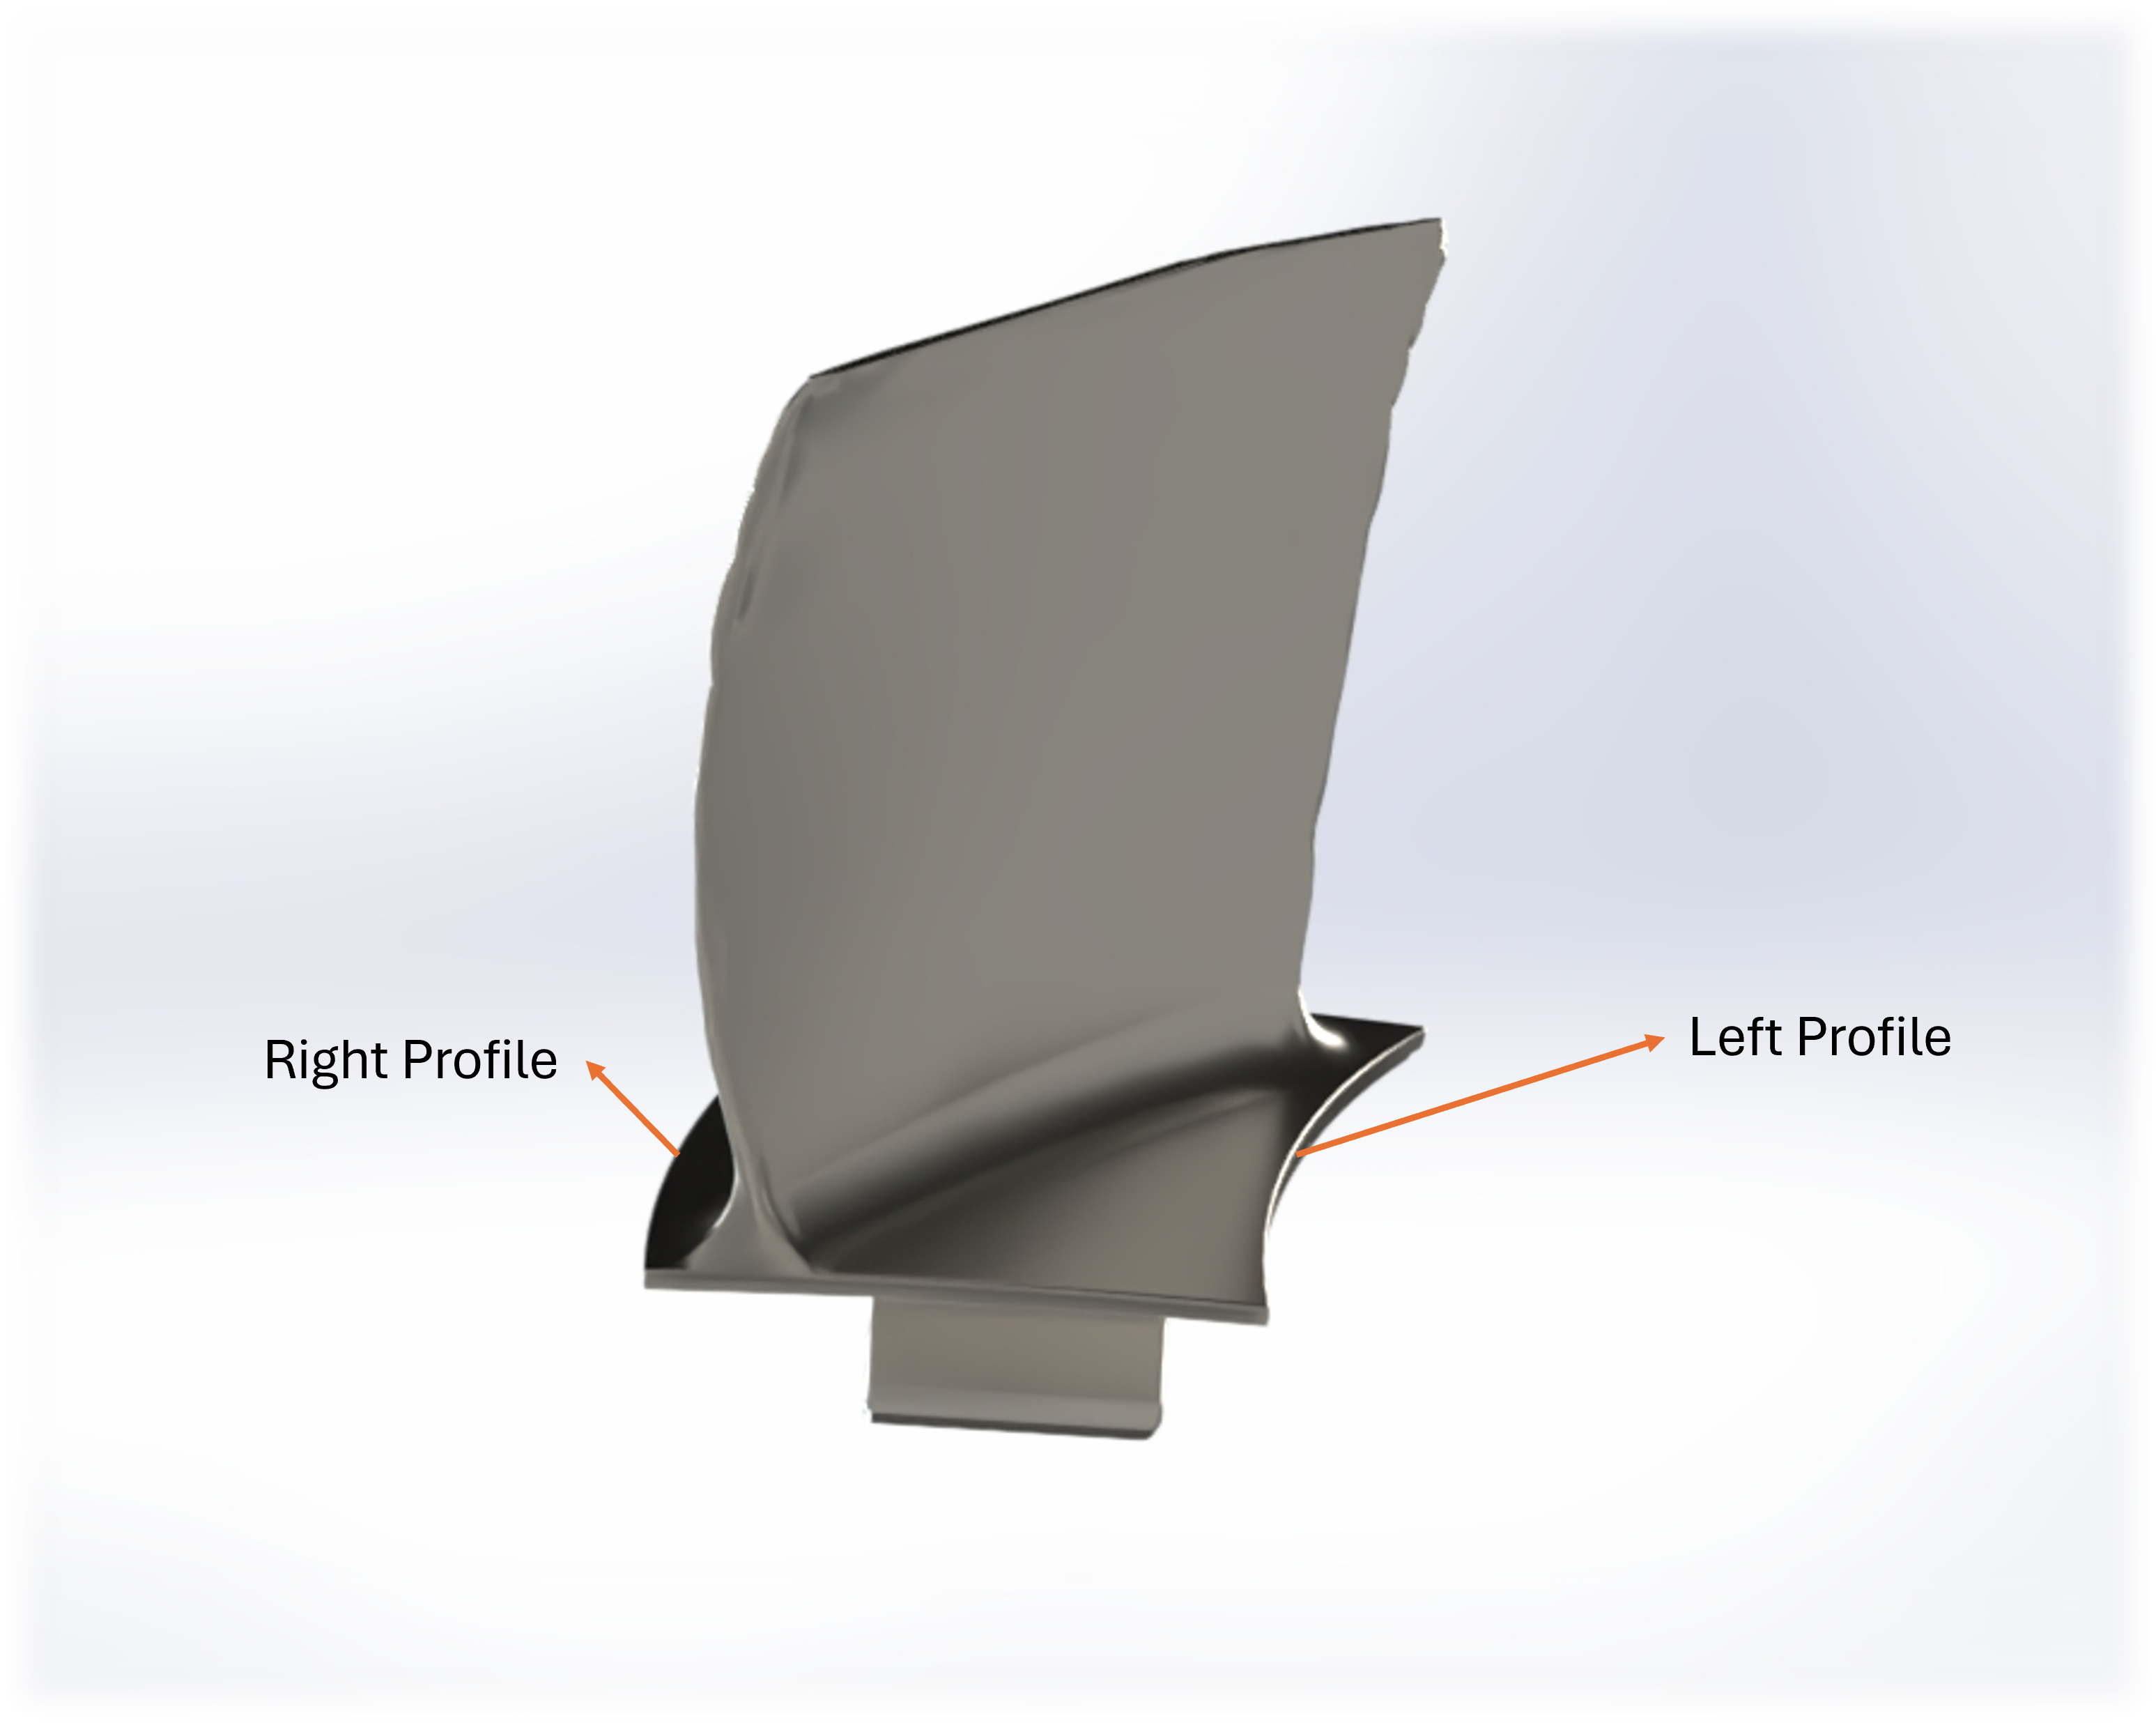
\includegraphics[width=0.5\textwidth]{Profiles}
    \caption{Contact zones identified by surface wear.}
    \label{fig:profiles}
\end{figure}


\subsubsection{Visual Inspection of Used Blades: Identifying Contact Zones}
\label{cha:iv}

Initially, to understand where contact between adjacent blades occurs, five used narrow-body blades and five used wide-body blades were randomly selected from a worn LEAP-1A engine. Since these blades had already been in operation, the wear marks left by contact made it possible to visually identify the contact zones. Evidence of contact was observed mainly at the extremities of both profiles, as shown in Figure~\ref{fig:contacto1}.

\begin{figure}[H]
    \centering
    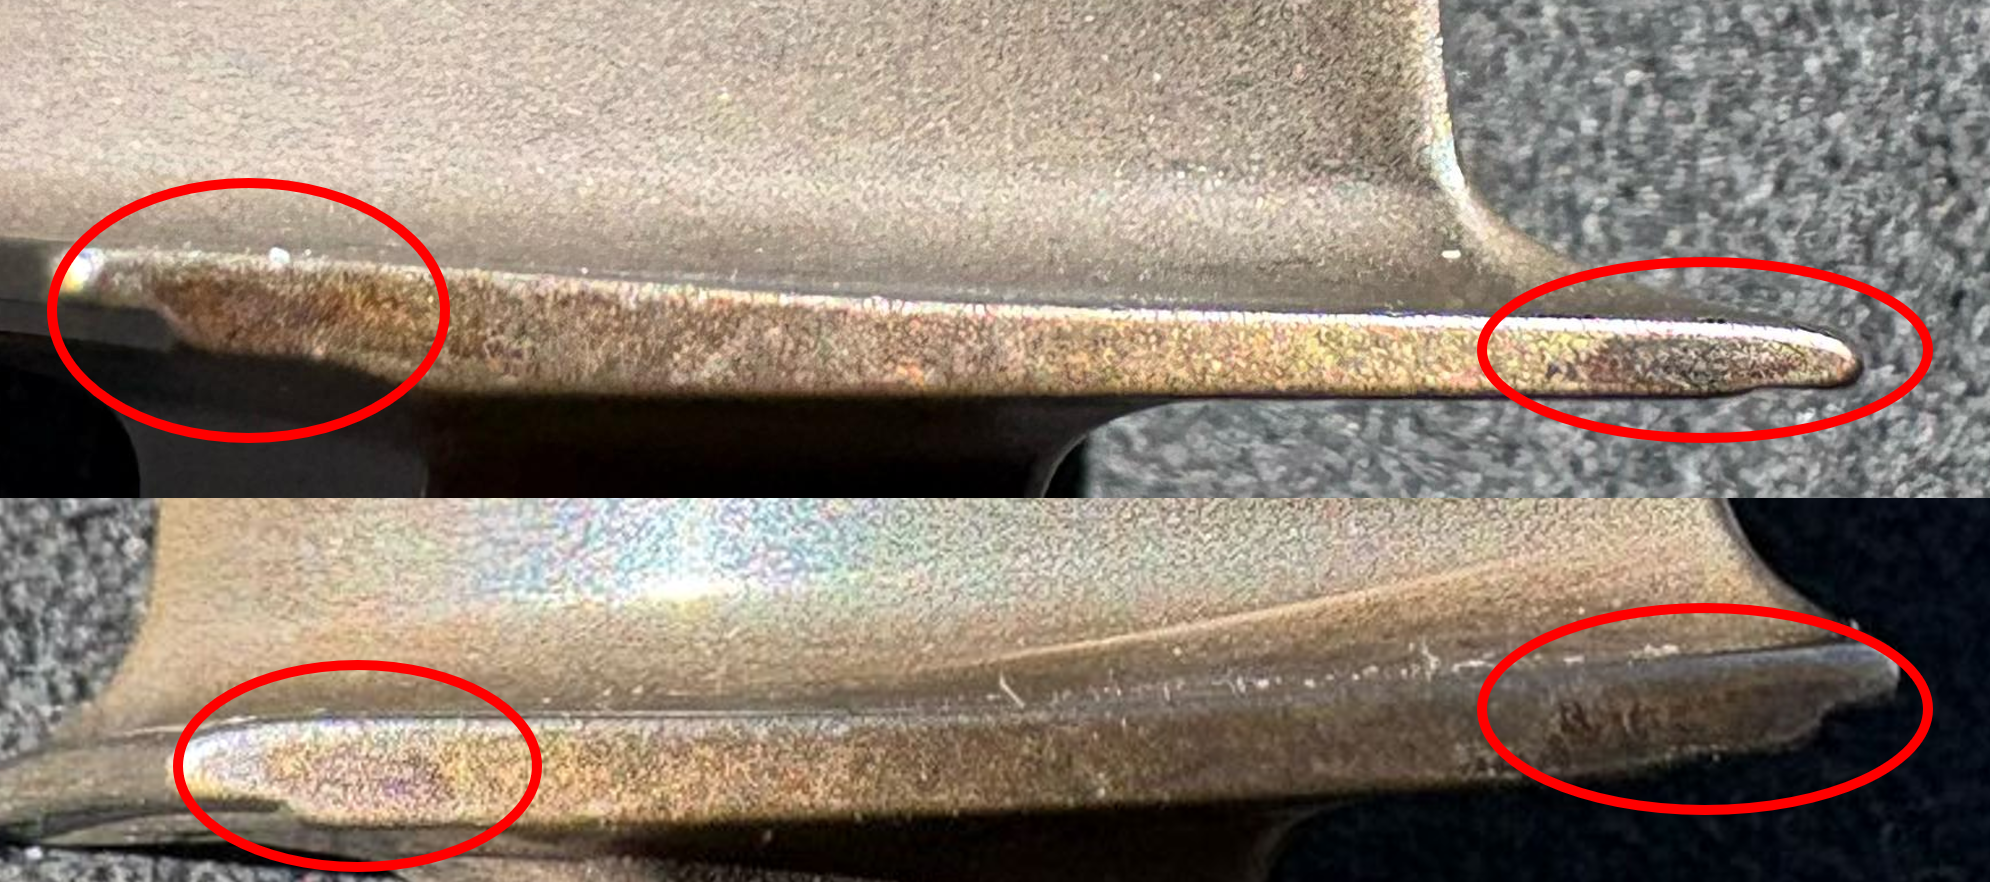
\includegraphics[width=0.5\textwidth]{Contacto1}
    \caption{Contact zones identified by surface wear.}
    \label{fig:contacto1}
\end{figure}

As shown in Figure~\ref{fig:contact}, this contact pattern consistently appears across all the selected blades, confirming the repeatability of the phenomenon. 

\begin{figure}[H]
    \centering
    \includegraphics[width=1\textwidth]{Pontos de Contacto}
    \caption{Contact zones identified by surface wear.}
    \label{fig:contact}
\end{figure}

The presence of consistent wear marks at the extremities of both profiles suggests that these are the actual contact points during blade assembly. This indicates that the platform clearance is effectively defined at these specific regions, making them the critical areas to consider when trying to understand how the assembly gap is established in practice.

\subsubsection{Dimensional Characterization of Blade Contact Surfaces Using CMM}
\label{cha:contactocmm}

As established in Section~\ref{subsec:desafios}, the dimensional tolerances required for blade manufacturing are extremely tight. For example, using the statistical tolerance model, the sixth stage of the HPC assembly demands a manufacturing tolerance of just \textbf{0.0645 mm} per blade. According to the metrology rule referred in \ref{subsec:equipment_validation}, the measurement uncertainty must be no greater than one-tenth of the tolerance. Therefore the required measurement uncertainty must be below \textbf{0.00645 mm (6.45~$\mu$m)}.

As previously discussed, the HandySCAN 3D scanner, although highly useful for general reverse engineering tasks, does not provide the necessary accuracy in critical areas such as blade edges or contact surfaces. Its resolution is insufficient to guarantee the precision needed for meaningful dimensional comparison at this scale.

For this reason, it became essential to resort to measurement by Coordinate Measuring Machine (CMM), which provides the required level of precision to properly define the problem dimensionally and allow for accurate blade analysis.

The CMM available at TAP ME normally offers a precision of 0.001 inches (25.4~$\mu$m). However, due to it being out of service at the time of this work, an alternative CMM was made available by the R\&D department of Hanon Systems. This machine operates with a precision of \textbf{1.6 + L/350~$\mu$m}, where \textit{L} is the length of the measured feature in millimetres.

For the measurements carried out on the contact profiles, this results in a measurement uncertainty of \textbf{1.6605~$\mu$m} for the left profile and \textbf{1.6614~$\mu$m} for the right profile---well within the required accuracy range for this analysis.


Before each measurement, the CMM performs an initial alignment process to establish the coordinate system (X, Y, and Z axes) and ensure that the fixation tool is correctly positioned. This procedure is illustrated in Figure~\ref{fig:CMMref}, which shows the alignment sequence in three steps.

In the first step (left image), the probe detects four points on the base of the fixation tool to define the initial plane — the YX plane.

Next (middle and right images), the machine scans four points on each lateral side of the fixation tool, resulting in eight points in total. Based on these, it calculates an intermediate surface that defines the YZ plane.

Finally, a single point is probed on the front face of the fixation tool (right image), allowing the system to determine the XZ plane and complete the coordinate setup.

While this method ensures consistency in positioning, it also presents a limitation: the alignment is referenced to the fixation tool rather than the blade itself. As a result, slight geometric deviations between individual blades may go unnoticed, reducing the accuracy of contact surface comparisons.

In this analysis, the same ten randomly selected sixth stage blades previously examined for surface wear — five narrow-body and five wide-body — were measured to capture detailed geometric data from the contact zones and assess part-to-part variation.

The resulting coordinate system, defined through this alignment procedure, is represented in Figure~\ref{fig:Eixos}, which was extracted from the CMM simulation software and visually illustrates the orientation of the X, Y, and Z axes relative to the fixture.


\begin{figure}[H]
    \centering
    \includegraphics[width=1\textwidth]{CMMref}
    \caption{Contact zones identified by surface wear.}
    \label{fig:CMMref}
\end{figure}

\begin{figure}[H]
    \centering
    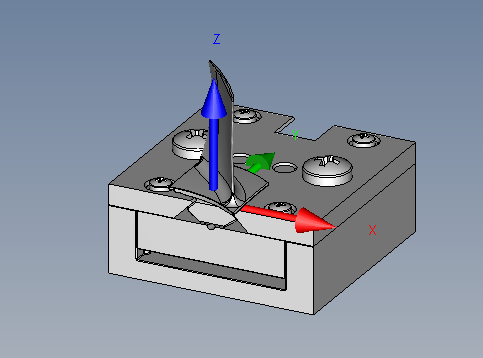
\includegraphics[width=0.6\textwidth]{Eixos}
    \caption{Contact zones identified by surface wear.}
    \label{fig:Eixos}
\end{figure}

The CMM measurement procedure consisted of single passes along the contact profiles. For each blade, the probe performed three scan paths: one on the left profile and one on the right profile with 400 points each, and two additional passes on the left profile at different heights. These dense point clouds allowed for a detailed reconstruction of the contact surface geometry.
Additionally, with the last two passes the system estimated the angle of the contact profile within the YZ plane to better understand the surface orientation. All individual measurements are presented in the annex, and the measured curvature radii are summarized in the following table.

\begin{table}[H]
    \centering
    \caption{CMM measured radii at left and right profiles for Narrow and Wide Body blades.}
    \begin{tabular}{ccc|ccc}
    \hline
    \multicolumn{3}{c}{\textbf{Narrow Body Radius (mm)}} & \multicolumn{3}{c}{\textbf{Wide Body Radius (mm)}} \\ \hline
    \textbf{Blade N$^{\circ}$} & \textbf{Left Profile} & \textbf{Right Profile} & \textbf{Blade N$^{\circ}$} & \textbf{Left Profile} & \textbf{Right Profile} \\ \hline
    1 & 30.7734 & 30.548  & 6 & 30.6168 & 30.6588 \\
    2 & 30.7584 & 30.545  & 7 & 30.5421 & 30.6623 \\
    3 & 30.7627 & 30.5403 & 8 & 30.5850 & 30.6342 \\ 
    4 & 30.7451 & 30.5411 & 9 & 30.5942 & 30.6323 \\ 
    5 & 30.7355 & 30.5327 & 10 & 30.6379 & 30.6614 \\ \hline
     & \textbf{Avg} 30.7550 & \textbf{Avg} 30.5414 & & \textbf{Avg} 30.5952 & \textbf{Avg} 30.6498 \\ \hline
    \end{tabular}
\end{table}
    
\begin{table}[H]
    \centering
    \caption{Summary of average and variation between maximum and minimum CMM-measured radii.}
    \label{tab:radii}
    \begin{tabular}{l|cc|cc}
        \hline
        \textbf{} & \multicolumn{2}{c|}{\textbf{Narrow Body (mm)}} & \multicolumn{2}{c}{\textbf{Wide Body (mm)}} \\ \hline
        \textbf{Profile} & \textbf{Left} & \textbf{Right} & \textbf{Left} & \textbf{Right} \\ \hline
        Average Radius & 30.7550 & 30.5414 & 30.5952 & 30.6498 \\
        Max-Min Variation & 0.0379 & 0.0153 & 0.0958 & 0.0300 \\ \hline
    \end{tabular}
\end{table}

Based on the results presented in Table~\ref{tab:radii}, the average values of the measured radii for each profile were defined as the nominal dimensions to be used in the blade model. The corresponding variations between the maximum and minimum values measured for each profile are considered representative of the dimensional tolerance associated with each nominal value. This approach ensures that the nominal model reflects the actual manufacturing variability observed across the sampled blades.

Additionally, as shown in the reports presented in the appendix and previously referenced, these measurements also aimed to estimate the angle of the contact profile within the YZ plane. However, due to the complex geometry and the limited thickness available for probing, the resulting values showed significant variation between blades.
This results are presented in Table~~\ref{tab:angulos}

\begin{table}[H]
    \centering
    \caption{Estimated angles of the contact profiles within the YZ plane (in degrees).}
    \label{tab:angulos}
    \begin{tabular}{c|c}
        \hline
        \textbf{Left Profile Angle ($^{\circ}$)} & \textbf{Right Profile Angle ($^{\circ}$)} \\ \hline
        -23.0719 & -34.9658 \\
        -31.6433 & -34.7307 \\
        -36.5751 & -36.2302 \\
        -35.0147 & -37.0324 \\
        -38.9593 & -32.0996 \\ \hline
    \end{tabular}
\end{table}

These results are presented in Table~\ref{tab:angulos}, which highlights the lack of consistency between the measured angles. Given this high variability, it was concluded that these values cannot be reliably used to define a nominal model for the contact profile geometry. Therefore, angle estimation was excluded from the subsequent dimensional analysis.

In the following chapters, if angle measurement becomes necessary, the measurement procedure will need to be revisited. This may involve using different probe paths or adopting a more suitable strategy to capture the angular orientation of these narrow surfaces with greater repeatability.
